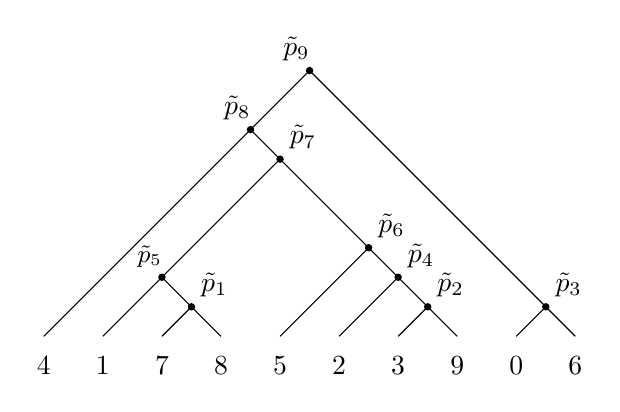
\begin{tikzpicture}[scale=1.5]
  \draw (0,0) -- (2.25,2.25);
  \draw (2.25,2.25) -- (4.5,0);
  \draw (2,1.5) -- (0.5,0);
  \draw (1.25,0.25) -- (1,0);
  \draw (1,0.5) -- (1.5,0);
  \draw (3.25,0.25) -- (3,0);
  \draw (4.25,0.25) -- (4,0);
  \draw (1.75,1.75) -- (3.5,0);
  \draw (3,0.5) -- (2.5,0);
  \draw (2.75,0.75) -- (2,0);
  
  \filldraw[black] (1.75,1.75) circle (0.75pt) node[label={[anchor=south east]0.1mm:$\tilde{p}_{8}$}]{};
  \filldraw[black] (2.25,2.25) circle (0.75pt) node[label={[anchor=south east]0.1mm:$\tilde{p}_{9}$}]{};
  \filldraw[black] (3.25,0.25) circle (0.75pt) node[anchor=south west]{$\tilde{p}_{2}$};
  \filldraw[black] (4.25,0.25) circle (0.75pt) node[anchor=south west]{$\tilde{p}_{3}$};
  \filldraw[black] (1.25,0.25) circle (0.75pt) node[anchor=south west]{$\tilde{p}_{1}$};
  \filldraw[black] (1,0.5) circle (0.75pt) node[label={[anchor=south east]0.1mm:\small $\tilde{p}_{5}$}]{};
  
  \filldraw[black] (2,1.5) circle (0.75pt) node[anchor=south west]{$\tilde{p}_{7}$};
  \filldraw[black] (3,0.5) circle (0.75pt) node[anchor=south west]{$\tilde{p}_{4}$};
  \filldraw[black] (2.75,0.75) circle (0.75pt) node[anchor=south west]{$\tilde{p}_{6}$};
  
  \draw[black] (0,-0.25) node{$4$};
  \draw[black] (0.5,-0.25) node{$1$};
  \draw[black] (1,-0.25) node{$7$};
  \draw[black] (1.5,-0.25) node{$8$};
  \draw[black] (2,-0.25) node{$5$};
  \draw[black] (2.5,-0.25) node{$2$};
  \draw[black] (3,-0.25) node{$3$};
  \draw[black] (3.5,-0.25) node{$9$};
  \draw[black] (4,-0.25) node{$0$};
  \draw[black] (4.5,-0.25) node{$6$};
\end{tikzpicture}


%%% Local Variables:
%%% mode: latex
%%% TeX-master: "main"
%%% End:
